\section{Indgangsvinkel}
\label{DatabehandlingRIndgangsvinkel}
%
I dette afsnit analyseres resultaterne med udgangspunkt i de tre forskellige indgangsvinkler robotten havde til testpersonerne i testen og hvis testpersonerne selv henvendte sig. De forskellige indgangsvinkler fremgår af \autoref{tab:RDistance}, hvor antallet af testpersoner ligeledes er opgivet. 

Det undersøges, hvordan robottens indgangsvinkel for henvendelse påvirker de rejsendes oplevelse af robotten ved at undersøge, hvordan resultaterne ændrer sig afhængigt af de tre forskellige indgangsvinkler samt testpersonernes egen henvendelse. Det er et \textit{Between-subject} design, da hver testperson kun har oplevet robotten i én af indgangsvinklerne eller selv henvendt sig, og svaret ud fra dette.
%
\begin{table}[H]
\centering
\begin{tabular}{c|c}
Indgangsvinkel & Antal testpersoner \\ \hline
Venstre (1) & 4    \\ \hline
Forfra (2) & 18    \\ \hline
Højre (3) & 8     \\ \hline
TP henvender sig (4) & 13 \\
\end{tabular}
\caption{Oversigt over antallet af testpersoner (TP) til hver af de tre indgangsvinkler robotten havde samt hvis testpersonerne selv henvendte sig.}
\label{tab:RDirection}
\end{table}
\noindent
%
Ud fra \textit{Scree}-plottet på \autoref{fig:Direction-Scree} fremgår det at cirka 60 \& af variansen kan forklares ud fra den første \textit{Principal Component} (PC) og 90 \% af variansen kan forklares ud fra to PCs, hvor PC2 bidrager med cirka 30 \%. Gøres der brug af alle tre PCs forklares 100 \% af variationen. 
%
\begin{figure}[H]
\centering
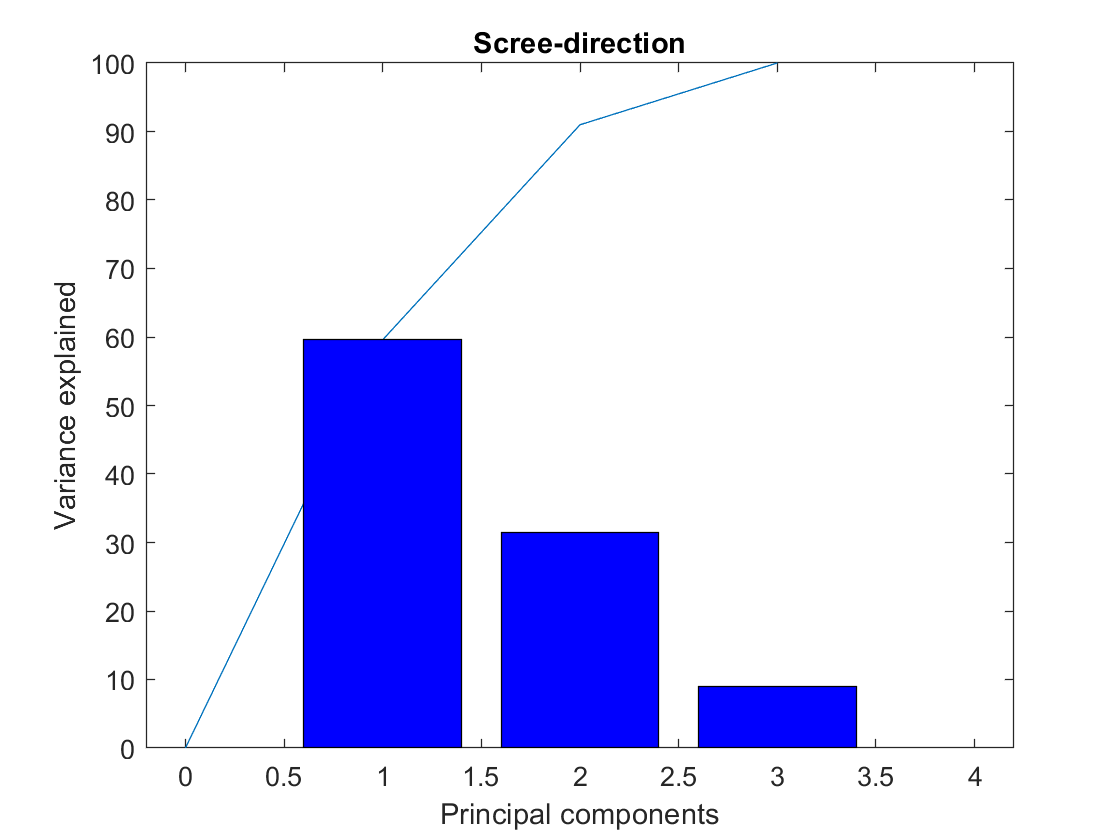
\includegraphics[width=\textwidth]{Figure/DatabehandlingSkalaer/PCAfigures/Direction-Scree.png}
\caption{\textit{Scree}-plot, hvorpå sammenhængen mellem antallet af \textit{Principal Components} og \textit{Variance Explained [\%]} fremgår.}
\label{fig:Direction-Scree}
\end{figure}
\noindent
% 
Ud fra \textit{Score}-plottet på \autoref{fig:Direction-Score} fremgår det, at der generelt er en del spredning mellem resultaterne ud fra de tre forskellige indgangsvinkler, hvilket foreskriver, at de tre indgangsvinkler ikke umiddelbart har ens karakteristikas. Dog ligger \textit{Kommer selv}, svarende til at testpersonerne selv henvendte sig til robotten, meget tæt på \textit{Forfra}, hvilket afspejler lignende karakteristikas for de to \textit{scores}. 
%
\begin{figure}[H]
\centering
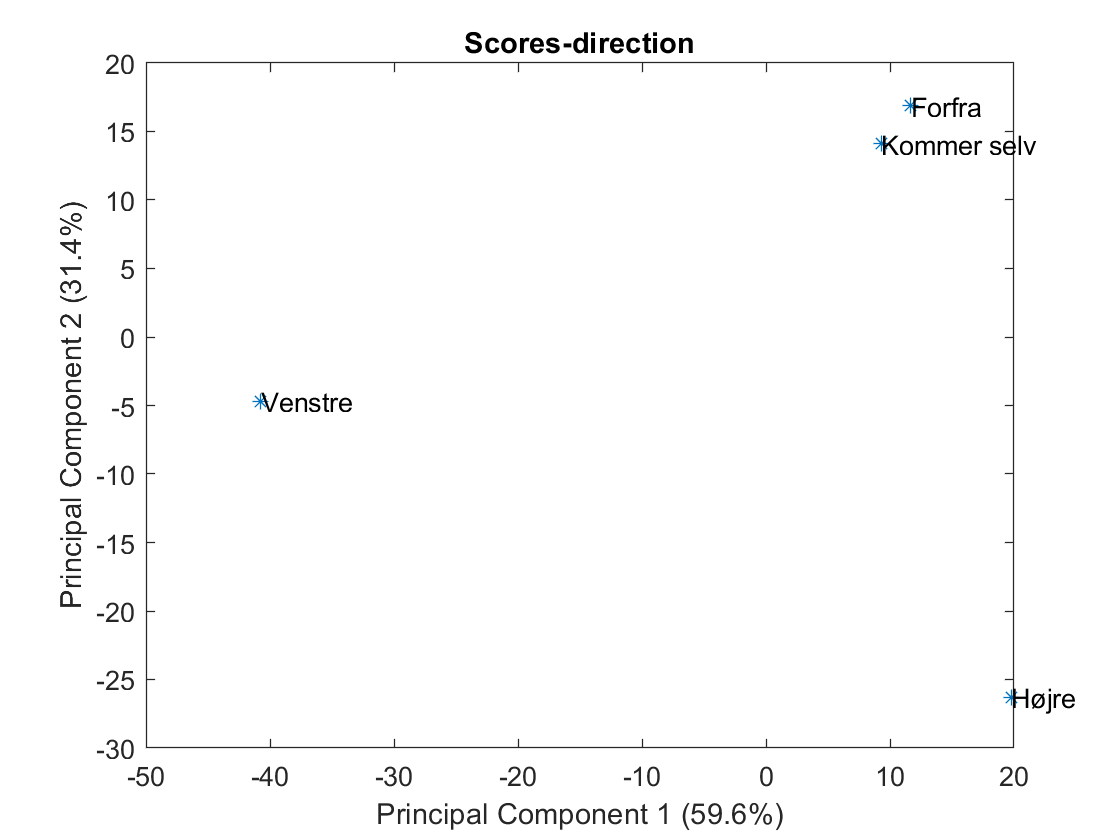
\includegraphics[width=\textwidth]{Figure/DatabehandlingSkalaer/PCAfigures/Direction-Scores}
\caption{\textit{Score}-plot for PC1 og PC2 i forhold til de tre indgangsvinkler robotten henvendte sig til testpersonerne med samt hvis testpersonerne selv henvendte sig.}
\label{fig:Direction-Score}
\end{figure}
\noindent
%
Ud fra \textit{Bi}-plottet på \autoref{fig:Direction-Biplot}, hvorpå \textit{loadings} og \textit{scores} for hver parameter er præsenteret, fremgår det at SQ10, vedrørende hvor tryg testpersonerne er ved robotten, forklare den største varians for PC1. For PC2 fremgår det, at både SQ1, vedrørende skærmens reaktion, SQ20, vedrørende hvor sej robotten opleves, samt SQ22, vedrørende hvor sjov robotten opleves, forklarer størstedelen af variansen. Da den forklaret varians fra SQ5, vedrørende robottens afstand, SQ6, vedrørende robottens hastighed, SQ7, vedrørende robottens højde, samt SQ16, vedrørende hvor irriterende robotten opleves, er relativt lille, vil disse parametre ikke blive yderligere beskrevet medmindre de indgår i en korrelation med en mere betydende parameter.  

I forhold til korrelationen mellem parametrene, fremgår det at SQ18, vedrørede hvor spændende robotten opleves, og SQ20, vedrørende hvor sej robotten opleves, har en positiv korrelation. Den positive korrelation er gennemgående for flere af parametrene, SQ8, vedrørende hvorvidt testpersonerne føler at robotten kan hjælpe dem, og SQ10, vedrørende hvor tryg testpersonerne er ved robotten, korrelerer ligeledes.  




SQ8 + SQ10 korrelation
SQ9 + SQ14 korrelation
SQ4 + SQ13 korrelation 
SQ1 + SQ16 korrelation
SQ5 + SQ7 + SQ17 korrelation

SQ1 + SQ12 negativ korrelation
SQ21 + SQ22 negativ korrelation
SQ9 og SQ14 + SQ8 +SQ10 negativ korrelation
SQ6 + SQ23 negativ korrelation



%
\begin{figure}[H]
\centering
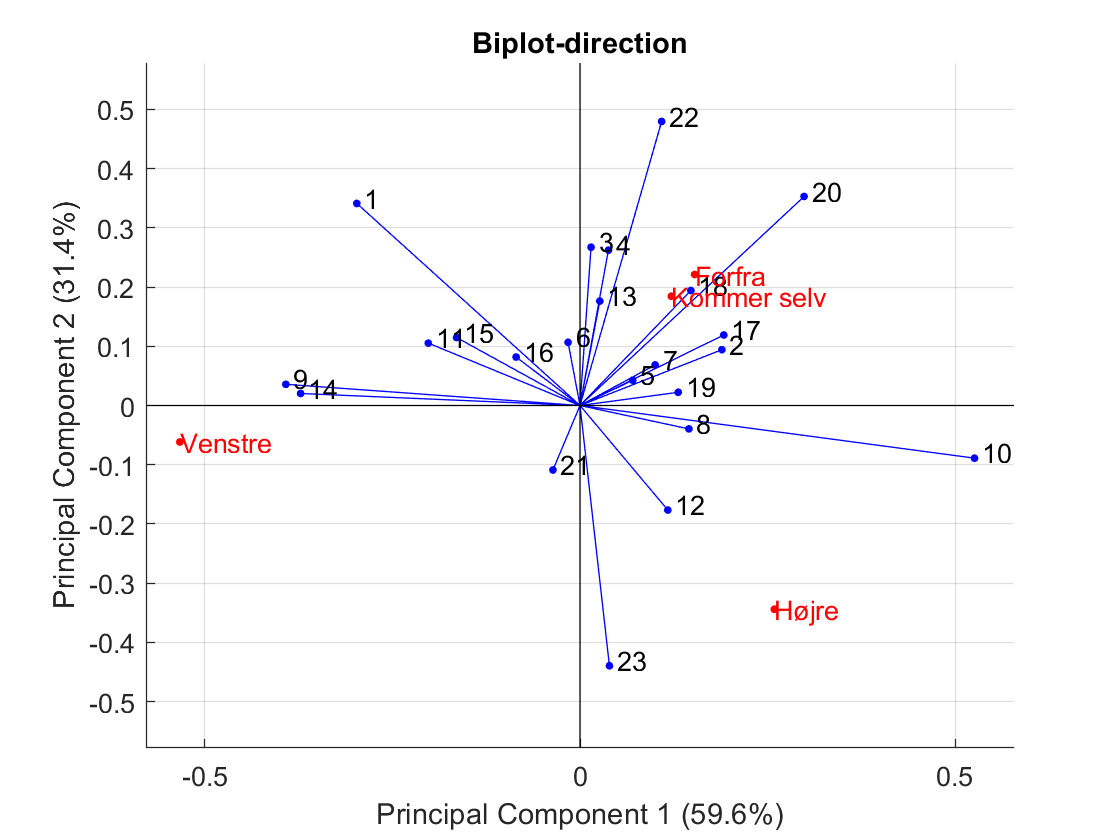
\includegraphics[width=\textwidth]{Figure/DatabehandlingSkalaer/PCAfigures/Direction-Biplot.png}
\caption{\textit{Bi}-plot med både \textit{loadings} (angivet med blå) og \textit{scores} (angivet med rød) fremgår i forhold til robottens indgangsvinkel.}
\label{fig:Direction-Biplot}
\end{figure}
\noindent
%

TABEL MED LOADINGS
%
\begin{table}[H]
\centering
\begin{tabular}{c|c|c|c}
    & PC1 (59.6\%)    & PC2 (31.4\%)    & PC3 (9\%)       \\ \hline
SQ1  & -0.2974         & 0.3412          & -0.2362         \\ \hline
SQ2  & 0.1890          & 0.0942          & -0.1122         \\ \hline
SQ3  & 0.0147          & 0.2673          & -0.0454         \\ \hline
SQ4  & 0.0379          & 0.2624          & 0.2993          \\ \hline
SQ5  & 0.0702          & 0.0427          & 0.0823          \\ \hline
SQ6  & -0.0159         & 0.1067          & 0.0165          \\ \hline
SQ7  & 0.1001          & 0.0686          & -0.0203         \\ \hline
SQ8  & 0.1451          & -0.0395         & 0.0291          \\ \hline
SQ9  & -0.3921         & 0.0358          & 0.0498          \\ \hline
SQ10 & \textbf{0.5258} & -0.0889         & -0.1395         \\ \hline
SQ11 & -0.2022         & 0.1053          & 0.3059          \\ \hline
SQ12 & 0.1170          & -0.1765         & 0.2387          \\ \hline
SQ13 & 0.0264          & 0.1764          & -0.4342         \\ \hline
SQ14 & -0.3724         & 0.0203          & 0.1812          \\ \hline
SQ15 & -0.1644         & 0.1147          & -0.2624         \\ \hline
SQ16 & -0.0851         & 0.0818          & 0.0851          \\ \hline
SQ17 & 0.1916          & 0.1191          & -0.1870         \\ \hline
SQ18 & 0.1478          & 0.1942          & 0.0192          \\ \hline
SQ19 & 0.1309          & 0.0223          & 0.2178          \\ \hline
SQ20 & 0.2987          & 0.3530          & \textbf{0.4448} \\ \hline
SQ21 & -0.0361         & -0.1089         & 0.2298          \\ \hline
SQ22 & 0.1088          & \textbf{0.4797} & -0.1187         \\ \hline
SQ23 & 0.0392          & -0.4395         & -0.1192        
\end{tabular}
\caption{Indgangsvinkel}
\label{tab:LoadingsIndgangsvinkel}
\end{table}
\noindent
%



TIL 3D plot 

SQ18 SQ20 er ikke positiv korrelation 
SQ13 + SQ4 er ikke positiv korrelation 
SQ1 + SQ16 er ikke positiv korrelation 
SQ7 + SQ17 er ikke positiv korrelation 
SQ5 + SQ17 er ikke positiv korrelation 

SQ2 + SQ7 korrelation


SQ21 + SQ22 er ikke negativt korrelation 

SQ13 + SQ21 er negativt korrelation



\subsection{Tendenser i forhold til robottens afstand}
\label{DatabehandlingAfstandTendenser}